\section{Konklusjon og anbefalinger}
\label{sec:konklusjon}
%\textit{Kort oppsummering av den innsikt som er oppnådd som er aktuelt for videreføring i Fase II. Enkelt-resultater som kan tallfestes bør være med.\\
%\\
%NB: Vær konkret på dette punktet. Det er uinteressant \textbf{at} gruppen har oppnådd innsikt på det ene eller andre området. Det interessante er \textbf{hvilken} innsikt som er oppnådd. %\\
%\\
%Anbefalinger for videreføring, bruk og vedlikehold er også viktig å få med.}


\subsection{Videreutvikling}

\subsubsection{Maskenettverk}

Systemet har slik det er nå en stor svakhet: aktivitet detekteres kun fra en side av turbinen, som gjør at mange fugler ikke blir detektert. 
Det vil heller ikke oppdages om en fugl faktisk kolliderer med turbinen. 
Derfor vil det være anbefalt som en videreutvikling av systemet å utvide til en maskenettverk bestående av flere noder med hvert sitt kamera og prosesseringsenhet som vist i  \autoref{fig:maskenettverk}. 
Her har hver av nodene to-veis kommunikasjon med nabonoden og kan videresende data slik at alle noder kan kommunisere med hverandre. 
Dette gjør at node 1 og 3 fortsatt kan kommunisere med hverandre selv om node 2 feiler. 
En skisse av systemet i praksis rundt en vindturbin er vist i \autoref{fig:fraoven}. 
Om en fugl detekteres på en side av turbinen, men ikke på den andre, vil et varsel kunne sendes til et operatør som kan undersøke om noe har kollidert med turbinen.

\begin{figure}[!htbp]
  \centering
  \begin{minipage}[b]{0.45\textwidth}
    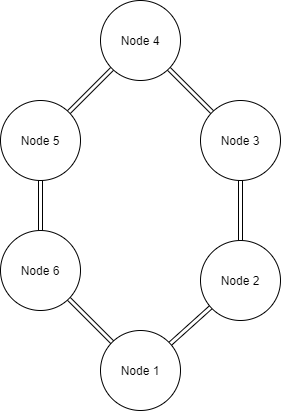
\includegraphics[width=\textwidth]{konklusjon/Mesh.png}
    \caption{Et tenkt maskenettverk for å dekke en hel vindturbin med seks noder. }
    \label{fig:maskenettverk}
  \end{minipage}
  \hfill
  \begin{minipage}[b]{0.45\textwidth}
    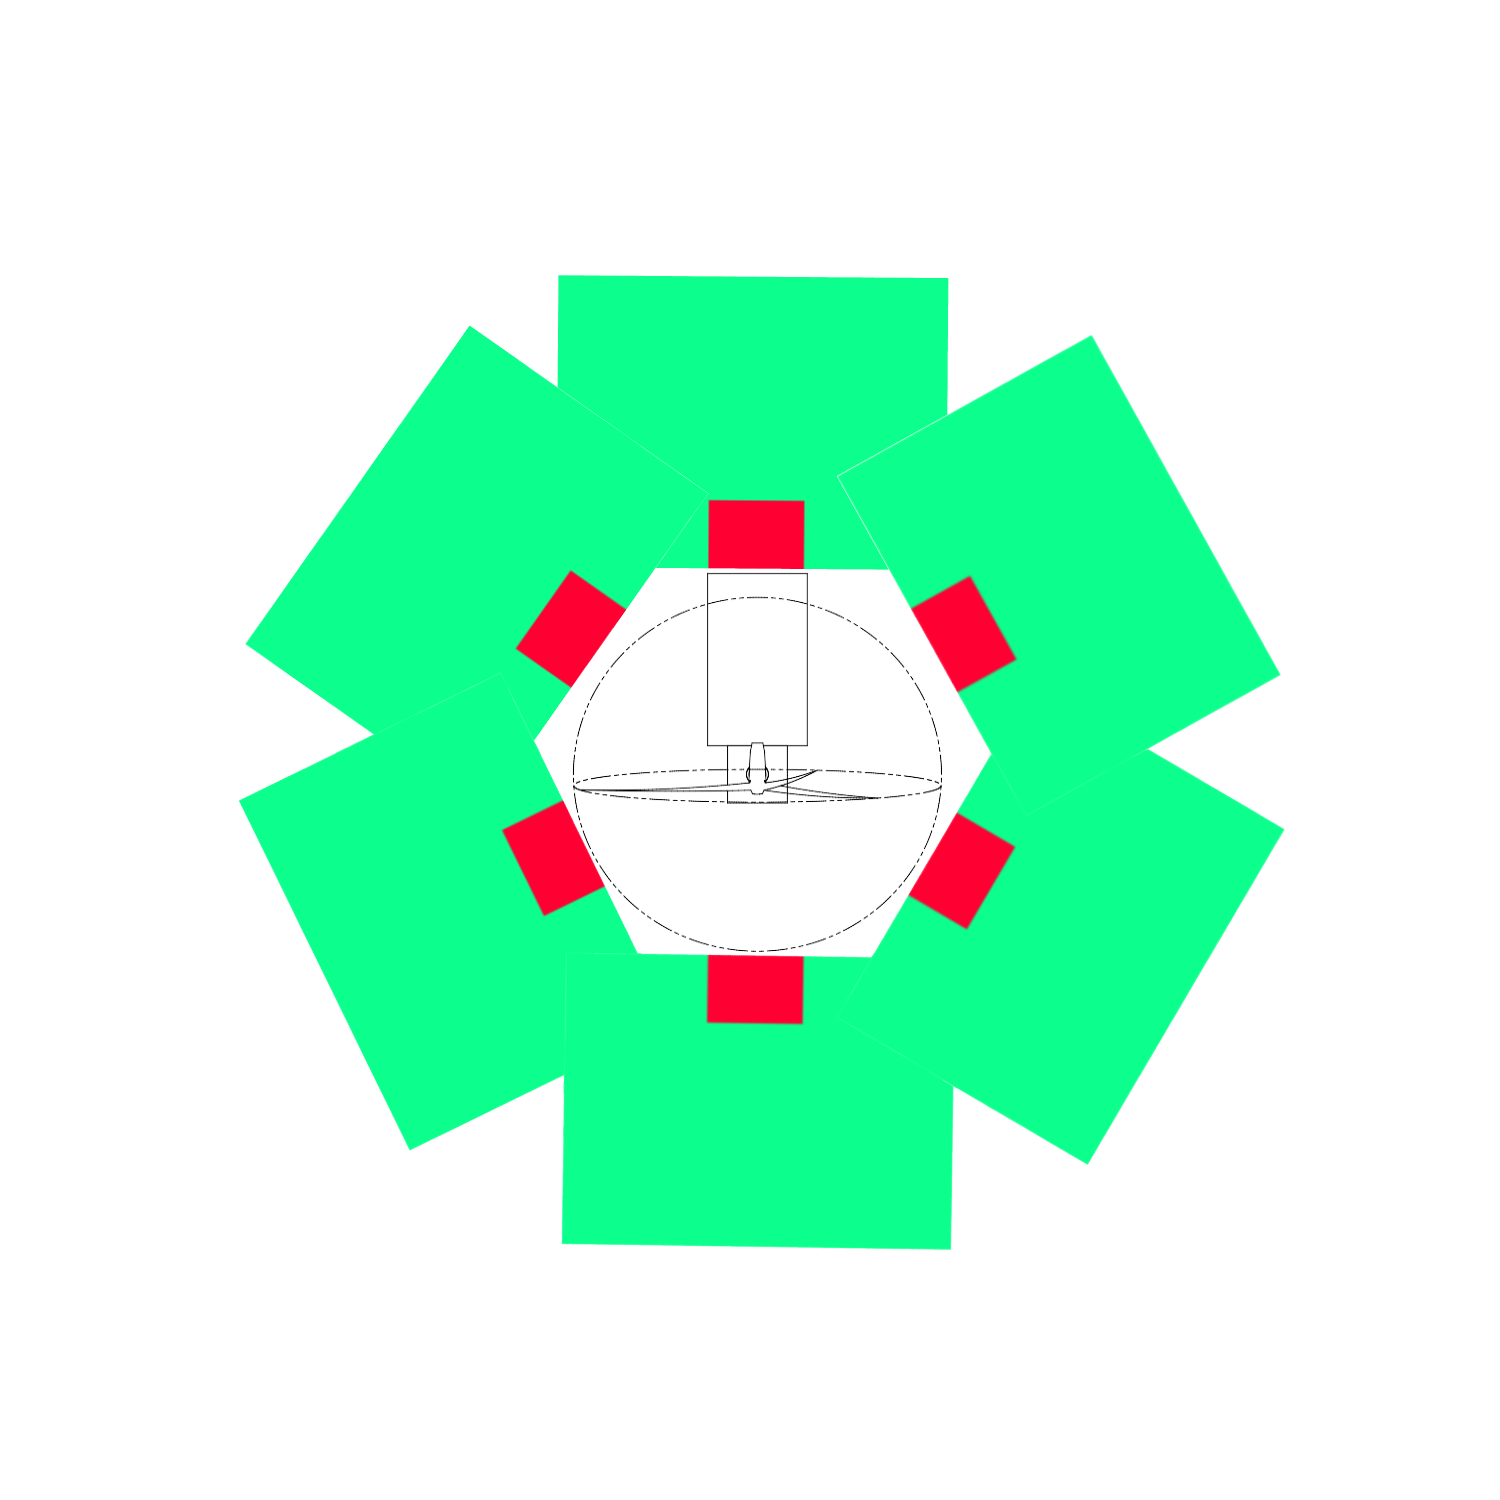
\includegraphics[width=\textwidth]{konklusjon/Nettverk.png}
    \caption{Konsept på hvordan seks kameraer kan detektere fugletrafikk inn mot en vindturbin fra alle retninger. Det grønne området er deteksjonsområdet og rødt er boksenes plassering.}
    \label{fig:fraoven}
  \end{minipage}
\end{figure}


Dette kan også hjelpe i områder uten vindkraftutbygging der man skal telle fugler på et større område. 
Dette vil gi en høyere sikkerhet i antall telte fugler, der en fugl som ikke blir telt av et kamera kan bli telt av et annet. 

Det er to grunner til at dette ikke har blitt gjennomført: penger og tid. 
Kameraet er den dyreste komponenten i systemet, der prisen for ett FLIR C3-kamera er på $\$700$. 
Det er også ansett som unødvendig å bruke tid på å utføre samme arbeid flere ganger i løpet av designprosessen til dette systemet.

\subsubsection{Oppgradering av IR-sensoren}
IR-kameraet vi bruker er et kommersielt kamera designet for å være brukervennlig. 
Dette skaper en del begrensninger rundt dataen vi får ut fra kameraet. 
Spesielt har den automatiske kalibreringen, diskutert i \autoref{sec:verifikasjon:kamera:kalibrering}, skapt problemer.  
I en videreutvikling burde dermed dette kommersielle kameraet byttes ut med kun en IR-sensor. 
Dette vil gi systemet mer kontroll over rådataen fra kameraet.
En IR-sensor med lengre rekkevidde og bedre oppløsning vil også gjøre det mulig å kartlegge arter og størrelser på fugler \cite{species}. 
Dette minsker behovet for et konvensjonelt kamera, som også ville vært avhengig av å ha god sikt. 
Kunnskap om art kan også i teorien kombineres med fuglens størrelse på skjermen for å slå fast avstand, gitt at fugler av den aktuelle arten har en kjent størrelse. 
Dette vil sannsynligvis være svært komplisert, og bør nok heller utføres med en avstandssensor.

\subsubsection{Ordinært bilde}
For enkelt å kunne sjekke om dataen fra fugletelleren er rimelig, kunne det vært gunstig å supplere IR-kameraet med et ordinært kamera som kun tar bilder når IR-kameraet detekterer en fugl.
Dette bilde kan så bli sendt til databasen, og gjort tilgjengelig på nettsiden.
Dette gjør det mulig for brukeren å enkelt dobbeltsjekke dataen, i tillegg til at det gjør det mulig å kartlegge art, enten automatisk ved hjelp av maskinlæring eller av et menneske. Dette vil kun fungere på dagtid og med god sikt.

\subsubsection{Egen strømforsyning}
For at brukeren skal ha større frihet ved plasseringen av produktet, er det viktig at det har sin egen strømforsyner og ikke er avhengig av å kobles til strømnettet.
Dette er spesielt viktig dersom man ønsker å overvåke et sted uten foreløpig installerte vindturbiner, da dette kan være langt unna eksisterende strømnett.
I en videreutvikling av produktet, vil det dermed være lurt å se på mulighetene for å koble produktet til et batteri, eventuelt supplert fra et lite solcellepanel eller liten vindturbin. 
 

\subsubsection{Programvare}
\todo{videreutvikkling av programmet noe maskinlæring kanskje}
\subsubsection{Filtrering}
\todo{skriv om filtrering under videreutvikkling}
Filteret fungertet sub-optimalt
Kombinere flere typer filter alla superposisjon hadde sikkert kunne gitt bedre resultat

\subsubsection{Blob-deteksjon og tracking}
\todo{skriv om blob-detection og tracking under videreutvikkling}
? 
fungerte tålelig bra? 
må kanskje se mer på feks når fugler krysser bak hverandre?
optimalisering av kode for å kjøre mer effektivt
optimalisering av tracking for å unngå situasjoner hvor den bruker for lang tid på en frame
andre ting? %Ser ut som om blob detection fungerer greit ved gode værforhold. Usikker på om dette kapittelet har noe for seg. Blir litt som å "klage" på at dette fikk vi ikke til. Optimalisering for eksempel er noe man alltid kan gjøre uavhengig av om produktet er ferdig eller ikke. 


\subsubsection{Nettside og database}

Videreutvikling av nettsiden og databasen vil kunne være å legge til flere spesialiserte grafer for forskjellige data. 
Dersom det blir behov for et maskenettverk vil det også måtte være nødvendig å legge til funksjonalitet for å kunne støtte dette. 
Det kan være et kart der du kan se de forskjellige systemene og statistikk for hver enkelt node. 

Databasen har en svakhet, den er relativt treg. Samtidig er den meget fleksibel. 
Det finnes flere løsninger som håndterer dette, men å gå over til en database som ikke er så fleksibel mot at den blir raskere er en mulighet. 


\subsection{Bruk}

Etter at systemet er satt ut på ønsket område, vil produktet automatisk registrere fugler og værdata uten ytterligere menneskelig interaksjon. 
Produktet er svært enkelt å sette opp, og krever kun tilgang til en vanlig stikkontakt og internett. 

Produktet er i utgangspunktet vedlikeholdsfritt.
Det vil allikevel kunne oppstå situasjoner der menneskelig interaksjon er nødvendig. 
Dette kan for eksempel være dersom kameralinsen blir blokkert av noe, eller pålen systemet står på velter. 

\subsection{Konklusjon}
Systemet bruker et IR-kamera, en prosesseringsenhet og bildebehandling for å detektere, telle og spore fugler i kameraets synsfelt. 
Systemet sender antall registrerte fugler sammen med værdata fra systemets egne sensorer til en database.
En nettside henter data fra databasen, og sorterer disse etter brukerens ønske. Treffraten på fugler er på $75\%$ i klart vær. \todo{Finn bedre def av treffrate?| er deteksjonsrate bedre?}
Systemet har noe lavere treffrate, altså andel suksessfulle tellinger av fugler, når det er skyer.
Dette kommer i hovedsak av den automatiske kalibreringen. 
%Samtlige systemkrav er tatt høyde for, men flere er ikke fullført som diskutert i  \autoref{sec:verifikasjon:kowona}.
Alle undersystemene fungerer, fra overvåking av fugleaktivitet og innsamling av værdata til presentering på en nettside.


\subsection{Takk}

Takk til Institutt for elkraftteknikk for lån av FLIR C3. 

Takk til vår faglige veileder Bjørn B. Larsen for god veiledning.